\documentclass[acmsmall,review,anonymous]{acmart}\settopmatter{printfolios=true,printccs=false,printacmref=false}
\acmJournal{PACMPL}
\acmVolume{1}
\acmNumber{OOPSLA} % CONF = POPL or ICFP or OOPSLA
\acmArticle{1}
\acmYear{2018}
\acmMonth{1}
\acmDOI{} % \acmDOI{10.1145/nnnnnnn.nnnnnnn}
\startPage{1}
\setcopyright{none}
\bibliographystyle{ACM-Reference-Format}
\citestyle{acmauthoryear}   %% For author/year citations
\usepackage{my_style}
\usepackage{listings, wrapfig,xspace}
\usepackage{paralist}
\usepackage{booktabs} % To thicken table lines

\lstset{language=R}
\definecolor{LightGray}{rgb}{.92,.92,.92}
\definecolor{Gray}{rgb}{.3,.3,.3}
\definecolor{DarkGray}{rgb}{.5,.5,.5}
\lstset{ %
  columns=flexible,
  captionpos=b,
  frame=single,
  framerule=0pt,
  tabsize=2,
  belowskip=0.5em,
  backgroundcolor=\color{LightGray},
  basicstyle=\small\ttfamily,
  emphstyle=,
  keywordstyle=,
  commentstyle=\color{Gray}\em,
  stringstyle=\color{Gray},
  numbers=left,
  showstringspaces=false
}
\lstdefinestyle{R}{ %
  language=R,
  morekeywords={assign, delayedAssign},
  deletekeywords={env, equal, c, runif, trace, args, exp, t, all},
  breaklines=true
}
\lstdefinestyle{Rin}{ %
  style=R,
  breaklines=false
}

\newcommand{\eg}{\emph{e.g.},\xspace}
\newcommand{\ie}{\emph{i.e.},\xspace}
\newcommand{\cf}{\emph{cf.}\xspace}

\newcommand{\PIR}{\textsf{PIR}\xspace}
\newcommand\pirI[1]{\mathtt{#1}}
\renewcommand{\c}[1]{{\lstinline[style=Rin]!#1!}\xspace}
\newcommand{\code}[1]{{\lstinline[style=Rin]!#1!}\xspace}
% Macros for type names from the old paper.
\newcommand{\attr}[2]{\ensuremath{#1_{\mathtt{#2}}}\xspace}
\newcommand{\attrclass}[3]{\ensuremath{#1^{\mathtt{#3}}_{\mathtt{#2}}}\xspace}
\renewcommand{\to}{\ensuremath{\rightarrow}\xspace}
\newcommand{\D}{\ensuremath{\small\vec{\mathtt D}}\xspace} % Double
\newcommand{\I}{\ensuremath{\small\vec{\mathtt I}}\xspace} % Integer
\renewcommand{\C}{\ensuremath{\small\vec{\mathtt C}}\xspace} % Character
\renewcommand{\L}{\ensuremath{\small\vec{\mathtt L}}\xspace} % Logical
\newcommand{\R}{\ensuremath{\small\vec{\mathtt R}}\xspace} % Raw
\newcommand{\X}{\ensuremath{\small\vec{\mathtt X}}\xspace} % Complex
\newcommand{\Y}{\ensuremath{\small\vec{\mathtt Y}}\xspace} % Symbol
\newcommand{\sY}{\ensuremath{\small{\mathtt Y}}\xspace} % Symbol
\newcommand{\sS}{\ensuremath{\small{\mathtt S}}\xspace} % S4
\newcommand{\sF}{\ensuremath{\small{\mathtt F}}\xspace} % Closure
\newcommand{\sE}{\ensuremath{\small{\mathtt E}}\xspace} % Env
\renewcommand{\R}{\ensuremath{\small\vec{\mathtt R}}\xspace} % Raw
\newcommand{\sN}{\ensuremath{\small{\mathtt N}}\xspace}     % Null
%\renewcommand{\l}{\ensuremath{\small L<?>}\xspace}     % List
\renewcommand{\l}{\ensuremath{\small\underline{\mathtt ?}}\xspace}     % List
\newcommand{\sD}{\ensuremath{\small{\mathtt D}}\xspace} % Double
\newcommand{\sI}{\ensuremath{\small{\mathtt I}}\xspace} % Integer
\newcommand{\sC}{\ensuremath{\small{\mathtt C}}\xspace} % Character
\newcommand{\sL}{\ensuremath{\small{\mathtt L}}\xspace} % Logical
\newcommand{\sX}{\ensuremath{\small{\mathtt X}}\xspace} % Complex
\newcommand{\sR}{\ensuremath{\small{\mathtt R}}\xspace} % Raw
\newcommand{\ANY}{\ensuremath{\small{\mathtt ?}}\xspace}     % Any
\newcommand{\lT}[1]{\ensuremath{\small\underline{\mathtt{#1}}}\xspace}     % list<T>
\newcommand{\M}[1]{\ensuremath{\attr{\vec{\tt #1}}{mat}}\xspace}     % matrix
\newcommand{\df}{\ensuremath{\attr{\l}{df}}\xspace}     % data.frame

\newcommand{\contractr}{\emph{contractr}\xspace} % contractr
\newcommand{\roxygen}{\emph{roxygen2}\xspace} % roxygen
\newcommand{\typetracer}{\emph{typetracer}\xspace} % typetracer
\newcommand{\rdt}{\emph{R-dyntrace}\xspace}
\newcommand{\covr}{\emph{covr}\xspace}




\begin{document}
\title{Designing Types for R, Empirically}

\newcommand{\NUMFUNCTIONS}{25,000\xspace}  %%% TODO auto-gen
\newcommand{\NUMPACKAGES}{412\xspace}  %%% TODO auto-gen
\newcommand{\PACKAGES}{412\xspace}  %%% TODO auto-gen
\newcommand{\genthat}{genthat\xspace}  %%% TODO auto-gen
\newcommand{\YEARS}{20\xspace} %%TODO fix
\newcommand{\PERCFAILEDASSERTIONS}{2\%\xspace}
\newcommand{\NUMPKGSEVAL}{7000\xspace} % autogenerate
\newcommand{\NUMASSERTIONS}{39210391\xspace} %autogenerate
\newcommand{\PROPFUNSFAILEDCHECK}{21.21\%\xspace}
\newcommand{\PROPFUNSFAILEDCHECKNOSTHREE}{15.48\%\xspace} 
\newcommand{\PROPARGSFAILINGASSERTS}{3.53\%\xspace} % autogen....

\begin{abstract}
The R programming language is widely used in a variety of domains for tasks
related to data science. R was designed to favor an interactive style of
programming with minimal syntactic and conceptual overhead. This design is
well suited to interactive data analysis, but a bad firt for tools such as
compilers or program analyzers which must generate performant code or catch
programming errors.  In particular, R has no type annotations, its
operations are dynamically checked at runtime. The starting point for our
work are the twin questions, \emph{what expressive power is needed to
  accurately type R code?} and \emph{which type system is the R community
  willing to adopt?} Both questions are difficult to answer without actually
designing a type system and attempting to convince users and package
developers to try the proposed system.  The goal of this paper is to provide
data that can feed into the design process. To this end, we perform a large
corpus analysis with aim to gain insights in the degree of polymorphism
exhibited by idiomatic R code and explore potential benefits that the R
community could accrue from even a simple type system.  As a starting point,
we infer type signatures for \NUMFUNCTIONS functions from \NUMPACKAGES
packages among the most widely used open source R libraries. The signatures
use a minimal type language with only basic types, vectors and classes.  We
implement a contract checker that can be used to validate the inferred type
signatures.
\end{abstract} \maketitle

\section{Introduction}

Our community builds, improves, and reasons about programming languages.  To
make design decisions that benefit users, we need to understand our target
language as well as the real-world needs it answers. Often, we can appeal to
our intuition, as many languages are intended for general purpose
programming tasks. Unfortunately, intuition may fail when looking at
domain-specific languages as these languages designed for a specific group
of users to solve very specific needs. This is the case of the data science
language R.

R and its ancestor S were designed, implemented, and maintained by
statisticians. Originally they aimed to be glue languages for reading data
and calling statistical routines written in Fortran. Over three decades they
became widely used across many fields for data analysis and visualization.
Modern R, as an object of study, is fascinating. It is a vectorized,
dynamically typed, lazy functional language with limited side-effects,
extensive reflective facilities and retrofitted object-oriented programming
support.

Many of the design decisions that gave us R were intended to foster an
interactive, exploratory, programming style. These include, to name a few,
the lack of type annotations, the ability to use syntactic shortcut, and the
automatic conversion between data types.  While these choices have led to a
language with a low barrier to entry---many data science educational
programs do not teach R itself but simply introduce some of its key
libraries---they have also created a language where errors can go
undetected.

Retrofitting a type system to the R programming language would increase our
assurance in the result of data analysis. But, we are faced with two
challenges. First, it is unclear what would be the \emph{right} type system
for a language as baroque as R. For example, one of the most popular data
type, the \code{data.frame}, is manipulated through reflective operations --
a data frame is a table whose columns can be added or removed on the fly.
Second, but just as crucially, designing a type system that will be adopted
would require overcoming some prejudices and educating large numbers of
users.

This paper is a data-driven study of what a type system for the R language
could look like. Our intention is to eventually propose changes to the
language, but we are aware that for any changes to be accepted by the user
community they must clearly benefit the language without endangering
backwards compatibility. Our goal is thus to find a compromise between
simplicity and usefulness; any proposed type system should cover common
programming idioms while remaining easy to learn and to use.




In order to do this, we need to understand the degree of polymorphism
present in R code, that is to say, how programmers leverage the dynamic
nature of R to write code that can accept arguments of different types.
This understanding will drive our design.

We propose to capture the degree of polymorphism present in R by means
of a dynamic analysis of widely used libraries. For each function call we
can record the types of its arguments and of its return value. This allows
us to observe how many different combination of types are accepted by any
given function. Unlike many other languages, R has a carefully curated
software repository called CRAN. To be deposited in CRAN, a package must
come with sample dataset, tests and executable use-cases. As part of normal
operations these tests are run regularly and failing packages are removed.
This allowed us to have access to \PACKAGES libraries and about an order of
magnitude more runnable scripts that exercise those libraries.

The contributions of this paper are thus as follows:
\begin{itemize}
\item A large-scale analysis of the polymorphism present in function
  signatures of \PACKAGES widely used and actively maintained R packages.
\item A tracing and analysis pipeline that extends a previously published
  test generation tool named \genthat.
\item A set of type annotations that captures how programmers use types
in existing R code.
\end{itemize}

One threat to validity of our work is that we rely on dynamic analysis, so
our conclusions are only as good as the coverage of the possibly function
behaviors. Previous work~\cite{issta18} reported that running all the
scripts that come with CRAN packages gives, on average, 68\% test coverage.
We attempted to mitigate the threat coming from the fact that only part of
the code is being exercised by manual analysis. It would be reasonable to
ask for confirmation of the data by static analysis of the code, but sound
static analysis of R is difficult because of the extensive use of reflective
features such as \code{eval} and of the ability to redefine the meaning of
operators such as \code{+} and \code{if}.  Another threat to validity is
that we only have access to code that has been deposited in the CRAN
repository. While this may bias our findings towards code written to be
reusable and, possibly, better engineered than typical user code. This is
also the code that would most benefit from type annotations.

%
\section{Background} %%%%%%%%%%%%%%%%%%%%%%%%%%%%%%%%%%%%%%%%%%%%%%%%%%%%%%%%%

In this section, we will introduce the R programming language, as well as
discuss the dynamic analysis framework we used as part of our initial
analysis.

%
%
\subsection{The R Programming Language}\label{sec:R}

Over the last decade, the R Project has become a key tool for implementing
sophisticated data analysis algorithms in fields ranging from Computational
Biology~\cite{R05} to Political Science~\cite{R:Keele:2008}. At the heart of
the R project is a \emph{vectorized, dynamic, lazy, functional,
  object-oriented} programming language with a rather unusual combination of
features~\cite{ecoop12} designed to ease learning by non-programmer and
enable rapid development of new statistical methods.  The language, commonly
referred to as R was designed in 1993 by Ross Ihaka and Robert
Gentleman~\cite{R96} as a successor to S~\cite{S88}.  First released in
1995, under a GNU license, R rapidly became the lingua franca for
statistical data analysis. Today, there are over 13,000 R packages available
from repositories such as CRAN and Bioconductor.  With 55 R user groups
world-wide, Smith~\cite{eco11} estimates that there are over 2 million
end-users.

As an introduction to R, consider the code snippet in Fig.~\ref{sample} from
a top-level interaction where the user defines a function \code{normSum}
that accepts vectors of integers, logicals, doubles and complex values and
normalizes the vector with respect to its sum and rounds the results. The
function definition does not require type annotations, and all operations
transparently work on vectors of any length and different types.

\begin{figure}[!hb]{\begin{lstlisting}
> normSum <- function( m )  round( m / sum(m), 2)
> normSum(c(1L,3L,6L))
[1] 0.1 0.3 0.6
> normSum(c(1.1,3.3,6.6))
[1] 0.1 0.3 0.6
> normSum(c(1.6,3.3,6.1))
[1] 0.15 0.30 0.55
> normSum(complex(r=rnorm(3),i=rnorm(3)))
[1] 0.49+0.21i 0.30-0.18i 0.22-0.03i
\end{lstlisting}}
\caption{Sample R code}\label{sample}
\end{figure}

In R, functions can be called with named parameters, arguments can have
default values, and R also support variable argument lists.  To illustrate
all of this in a single example, consider:

\begin{lstlisting}
f <- function(x, ..., y=3) x + y
\end{lstlisting}

\noindent
Function \k{f} can be called with a single argument \code{f(3)}, with named
argument \code{f(y=4,x=2)} and with a variable number of arguments,
\code{f(1,2,3,4,y=5)}, all of these calls will return \code{6}.

R has a number of features that are not crucial to the present
discussion. We will mention some of them here for completeness.  In R, data
structures are reference counted and have copy-on-write semantics, thus the
assignment \code{x[12]<-3} results in an update to a copy of \code{x} unless
the reference count on that object is 1.  This semantics gives R a
functional flavor while allowing updating in place within loops (the first
update copies, subsequent updates are performed on the copy). Arguments to
functions are evaluated only when needed, they are bundled in so-called
promises which package the original expression (as an abstract syntax tree, or AST), its environment
as well as the result of evaluating the expression. Promises can be
leveraged for meta-programming as it is possible to retrieve the text of a
promise and evaluate it in a different environment.


\subsubsection{Types of Data}
\label{subsubsec:backgroundtypes}

Before attempting to define a type system for R, we should understand the
different kinds of values that programs operate on.  As we will see
different notions of type may emerge depending on how granular we want to
be.

\renewcommand{\k}[1]{{\tt #1}\xspace}

R has one builtin notion of type that can be queried by the \k{typeof}
function. Figure~\ref{types} lists all of the builtin types that are
provided by the language. They are the possible return values of
\k{typeof}. There is no intrinsic notion of subtyping in R. But, in many
context a \k{logical} will convert to \k{integer}, and an \k{integer} will
convert to \k{double}.  Some off conversions can occur in corner cases, such
as \k{1<"2"} holds and \k{c(1,2)[1.6]} returns the first element of the
vector, as the double is converted to an integer. R does not distinguish
between scalars and vectors (they are all vectors), so \code{typeof(5) ==}
\code{typeof(c(5)) == typeof(c(5,5))} \code{ == "double"}. Finally all
vectorized data types have a distinguished missing value denoted by
\code{NA}. The default type of \code{NA} is \k{logical}. We can see that
\code{typeof(NA)=="logical"}, but NA inhabits every type:
\code{typeof(c(1,NA)[2])=="double"}.

\begin{wrapfigure}{r}{6.1cm}
\footnotesize\begin{tabular}{l|l@{}}\hline
\multicolumn{2}{l}{\bf Vectorized data types:}  \\\hline
\k{logical}   & vector of boolean values\\
\k{integer}   & vector of 32 bit integer values\\
\k{double}    & vector of 64 bit floating points\\
\k{complex}   & vector of complex values\\
\k{character} & vector of strings values\\
\k{raw}       & vector of bytes\\
\k{list}      & vector of values of any type\\\hline
\multicolumn{2}{l}{\bf Scalar data types:}\\\hline
\k{NULL}      &  singleton null value\\
\k{S4}        &  instance of a S4 class \\
\k{closure}   &  function with its environment\\
\k{environment}& mapping from symbol to value \\\hline
\multicolumn{2}{l}{\bf Implementation data types:}\\\hline
\multicolumn{2}{l}{\k{special},
\k{builtin},
\k{symbol},
\k{pairlist},
\k{promise}}\\
\multicolumn{2}{l}{
\k{language},
\k{char},
\k{...},
\k{any},
\k{expression},
}\\
\multicolumn{2}{l}{
\k{externalprt},
\k{bytecode},
\k{weakref}}\\\hline
\end{tabular}\caption{Builtin Types}\label{types}\end{wrapfigure}

With one exception all vectorized data types are monomorphic, the exception
is the \k{list} type which can hold values of any other type including
\k{list}. For all monomorphic data types, attempting to store a value of a
different type will cause a conversion. Either the value is converted to the
type of vector, or the vector is converted to the type of the value.

Scalar data types include the distinguished \k{NULL} value, which is also of
type \k{NULL}, instance of classes written using the S4~\footnote{put footnote on S4 here} object system,
closures and environments.  The implementation of R has a number of other
types that are mostly not used by user code, they are listed in
Figure~\ref{types} for reference.

Over the years, programmers have found the need for a richer type
structure and have added {\it attributes}. The best way to think of attributes is
as an optional map from name to values that can be attached to any object.
Attributes are used to encode various type structures. They can be queried
with functions such as \k{attributes} and \k{class}.
The addition of attributes lets programmers extend the set of types by
tagging data with user-defined attributes. For example, one could define a
vector of four values, \code{x<-c(1,2,3,4)} and then attach the attribute
\k{dim} with a pair of numbers as value: \code{attr(x,"dim")<-c(2,2)}.  From
that point, arithmetic functions will treat \k{x} as a 2x2 matrix. Another
attribute that can be set is the \k{class}.  This attribute can be bound to
a list of class names. For instance, \code{class(x)<-"human"}, set the class
of \k{x} to be \k{human}.  Attributes are thus used for object-oriented
programming. The S3 object system support single dispatch on the class of
the first argument of a function, whereas the S4 object system allows
multiple dispatch (on all arguments). Some of the most widely used data
type, such as data frames, leverage attributes. A data frame, for instance,
is a list of vectors with a class and a column name attribute.


%
%
\section{Project Corpus}\label{sec:corpus}

For this paper we have selected \CorpusLoadable packages consisting of
\CorpusRCodeRnd lines of R code and \CorpusNativeCodeRnd lines of native
code (C/C++/Fortran). Figure~\ref{fig:corpus} shows all the packages, the
size of the dots reflects the size of the project in terms of both R and
native lines of code\footnote{ Lines of source code reported excludes
  comments and blank lines, counted by \emph{cloc}, \cf
  \url{https://github.com/AlDanial/cloc}}, the x-axis indicates the
expression code coverage in percents and the y-axis gives the number of
reverse dependencies in log scale. Dotted lines indicate means.  Packages
with over \PackageSizeOutierRnd lines of code are annotated.

\begin{figure}[!h]  \centering
  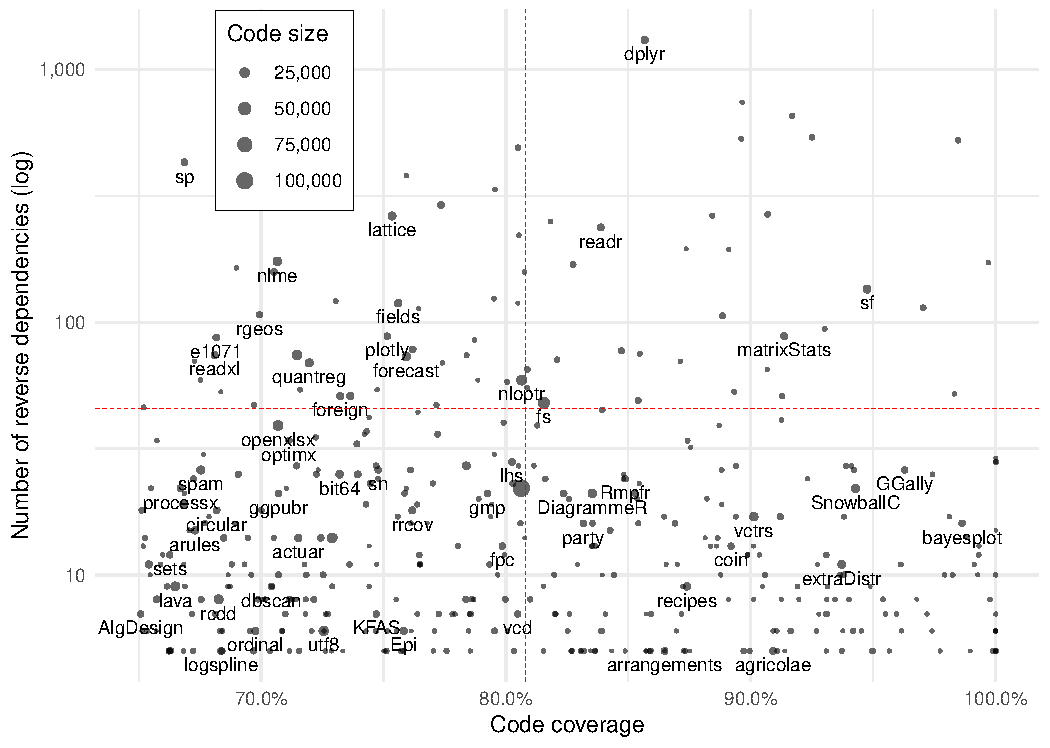
\includegraphics[width=.8\linewidth]{plots/corpus.pdf}
  \caption{Corpus overview}\label{fig:corpus}
\end{figure}

These packages come from the Comprehensive R Achive Network
(CRAN\footnote{\url{http://cran.r-project.org}}), the largest repository of
R code with over \AllCranRnd packages\footnote{CRAN receives about 6 new
  package submissions a day~\cite{Ligges2017}} containing over \AllRCodeRnd
and \AllNativeCodeRnd R and native code respectively. Unlike other open code
repositories like GitHub, CRAN is a curated repository. Each submitted
package must abide to a number of well-formedness rules that are
automatically checked asserting certain quality. Most relevant for this work
is that all of the runnable code (including code snippets from examples and
vignettes) is tested and only a successfully running package is admitted in
the archive.

We have downloaded and installed all available CRAN packages. Out of the
\AllCranRnd packages, we managed to install \AllLoadableRnd. The main reason
for this is that \rdt is based on R 3.5.0 and some of the packages are no
longer compatible with it. Some packages also require extra native
dependencies which were not present on our servers.  We have two criteria
for including a package into the corpus:
\begin{inparaenum}[(1)]
\item have runnable code that covers significant part of the package source
  code from which type signatures could be inferred, and
\item have some reverse dependencies that allows us to evaluate the inferred
  types on runnable code from these dependent packages.
\end{inparaenum}
The concrete thresholds were set to at least \ThresholdCodeCoverage of
expression coverage and at minimum \ThresholdRevdeps reverse dependencies.

The code coverage was computed for each package using
\covr\footnote{\url{https://github.com/r-lib/covr}}, the R code coverage R
tool.  The reverse package dependencies were extracted from the package
metadata using builtin function.

%
%
%
\section{Methodology}

In this section, we will describe our approach to data collection and
analysis through \typetracer, a dynamic analysis built in the \R-dyntrace
framework.  We will then describe the process by which we distill the rich
information we collect with \typetracer to more digestible ``types'', though
we discuss the precise details of our type annotation language in
Section~\ref{sec:types}.  Finally, we discuss \contractr, a package built in
R which supports our type language and can generate and check contracts for
function types.

%
\subsection{R-dyntrace}
R-dyntrace is a framework for performing dynamic analysis of R. It was designed
and used previously for a large-scale study of laziness in R~\cite{oopsla19} It
is an instrumented R Virtual Machine based on GNU-R version 3.5.0. It exposes
hooks from key points inside the R interpreter to which user defined callbacks
can be attached for gathering information about the program state at those
points. This information can be used to generate detailed program traces for
online or offline analysis. R-dyntrace provides hooks for function entry and
exit, S3/S4 dispatch, non-local jumps (because of longjumps in the R interpreter
on exceptions and other non-local returns), promise creation and forcing,
variable definition and mutation and garbage collection. garbage collection
entry and exit, function entry and exit.


%
%
\subsection{typetracer and Initial Analysis}

To help inform the design of our type system, and to ensure that it aligns
with the day-to-day usage of R, we performed a corpus analysis of some of
the most widely used R packages.  The corpus is discussed in detail in
Section~\ref{sec:corpus}.  We built \typetracer, our dynamic analysis, in
the R-dyntrace~\cite{oopsla19} dynamic analysis framework which is itself
built on a modified version of R targeting R version 3.5.0---we refer the
reader to Section~\ref{sec:r-dyntrace} for more details on the framework.

%
%
\subsubsection{Overview}
The goal of our analysis is to discover argument types for functions,
builtins, and specials (R functions such as \{, \code{if}, etc.).  First,
recall that R wraps arguments in promises (Section~\ref{sec:R}).  Naively
intercepting function calls and recording argument types would result in
incomplete data: While we can dig into promises without forcing them, if the
innermost value is an unevaluated expression we are unable to probe it
without evaluating it, which may alter program behaviour.  To circumvent
this obstacle, we instead intercept the forcing of promises: when a promise
is forced, we identify the surrounding call, collect the type of the value,
and add it to the call trace associated with the current function call.
Once function execution completes, we collect information about the return
value, add it to the call trace, and save the completed call trace to be
written out later.
%
%
\subsubsection{Type Information}
Once a value is obtained, either on function return or when an argument
promise is forced, we can probe it without interfering with program behaviour.
We query the value for the following information:

\begin{itemize}
\item the value's type tag according to R's runtime. R's runtime implements
  type tags as a typedef, e.g. \code{INTSXP} for integers, and, confusingly,
  \code{VECSXP} for lists;
\item its class, which is a list of string class names. Typically, the class
  of a value is held in an attribute with name ``class'', though some
  classes are blessed by the R runtime, such as matrix and array classes;
\item its attributes, a list of metadata attached to the value.
\end{itemize}

Now, depending on the value's type tag, we collect further information:

\begin{itemize}
\item For R's primitive types, we collect its dimension, and if it has a
  names attribute we collect the names as well;
\item For lists, we recursively collect the types of list elements;
\item For lists {\it with a names attribute}, we collect the names as well
  as the types of the slots that those names refer to (data.frames fall into
  this category);
\item For promises, we carefully dig into the promise value {\it without
  forcing it}, and collect information about the innermost value. If the
  innermost value is the unbound value, then the promise is an as-of-yet
  unevaluated expression. In this case, we do our best to guess the value of
  the unevaluated expression: if the expression is not a language
  expression, we collect information about it, otherwise we can say nothing
  without evaluating it and ascribe it type ``any''. \footnote{\AT{I think
      this is confusing, reword.}}
\end{itemize}

For vectors (and lists), we additionally iterate through the elements,
checking if the values are NA (resp. NULL); if none are NA (resp. NULL), we
ascribe the NA-free (resp. NULL-free) tag to the value.  Arguments that are
part of a function's varargs (denoted \ldots in function definitions) are
tagged as such and ignored, as varargs can contain anything (and their type
will be equivalent to and any-typed list).

Now that we've seen the high-level picture of our approach, we will elaborate on some key details and discuss particular challenges that we faced.

%
%
\subsubsection{Challenges}
\label{subsec:typetracer-challenges}

We grappled with a number of corner cases related to R's non-strict semantics.

\begin{itemize}

\item First, we wanted to ensure that \typetracer captured types for
  unevaluated arguments.  Unfortunately, not every argument of a function is
  necessarily used during every function execution, meaning that some
  arguments may remain unevaluated (as they are never forced), and there are
  a few reasons for this.

  One possibility is that the argument was simply unused given the control
  flow of this particular execution (e.g. if the argument is only needed in
  one branch of a conditional expression).  This mainly occurs when
  arguments have default values for some parameters that are not critical to
  every execution of the function.  In these cases, we still want to collect
  the type of the default value.

Another possibility is that a value is used {\it without being forced}, as
is the case when values are ``metaprogrammed''.
This is common practice in e.g. the \code{tidyverse}~\footnote{\AT{either talk about it here or in background}} ecosystem, as they use the metaprogramming capabilities of R to implement a DSL for data analysis.


To tackle possibly unevaluated arguments, we make an {\it initial guess} of function argument types on
function entry. Specifically, we collect types for argument default values, and
ascribe an ``unused'' type for unevaluated expressions.  If an argument
promise is later forced, we simply update the recorded type for the
argument.

\item Second, we wanted to account for formal arguments (arguments which are
  named in the function definition) which received no values when the function was called. This represents cases where a function was not called with all of its
  arguments, and no default value was specified for missing arguments. 
  We record a ``missing'' type for such argument.

There are two obvious ways to deal with missing arguments: type them as $\bot$
or as $\top$.  As we are performing a dynamic analysis based on package test
code, we conservatively type these arguments as $\top$, or \code{any}, as It is
impossible to know dynamically what all possible function behaviours are.
We discuss the prevalence of such any-typed arguments in
Section~\ref{sec:evaluation}.

\item Third, we had to contend with R's backend sometimes
  performing longjumps, which discards current R calls from the call stack.
  In order to ensure that call traces are not lost when a longjump occurs,
  \typetracer intercepts the unwinding process initiated by the longjump and
  mimics the functionality of the functions being exited.  The R-dyntrace
  framework supplies the return value during the unwinding process (if there
  is indeed such a value), so we can capture it, analyze it, and include it
  in the call trace.  In certain situations, however, no return value can be
  obtained (e.g. a longjump occurred as part of some error handling), and
  then we simply record a ``jumped'' return value, which we can deal with in
  post-processing.  
\end{itemize}

Having outlined these challenges, we will now explore the implementation of \typetracer in more detail.

%
%
\subsubsection{Select Details}

As mentioned, our analysis is built on the R-dyntrace framework.  R-dyntrace
is a very efficient instrumentation framework for R, which is built on a
modified version of the R runtime. 
% Our dynamic type analysis only needs to be run once, ever---from the analysis results, we synthesize function signatures which are passed along to later type-checking tools which do not rely on a heavily modified runtime.

We primarily rely on 8 R-dyntrace callbacks: \texttt{closure\_entry},
\texttt{closure\_exit}, \texttt{builtin\_entry}, \texttt{builtin\_exit},
\texttt{special\_entry},\texttt{special\_exit},
\texttt{promise\_force\_entry}, and \texttt{promise\_force\_exit}.  These
callbacks fire when closures, builtin, and special functions are entered and
exited, and before and after the forcing of promises.  The function-related
callbacks are used mainly for bookkeeping: the analysis is notified that a
closure, builtin, or special has been entered/exited by pushing/popping the
call onto a stack.  The calls themselves store a {\it call trace} object,
where we store the type information that we collect, populated with initial
guesses of argument types (as discussed in
Section~\ref{subsec:typetracer-challenges}).  
Also, recall that R can perform single or multiple dispatch on function arguments depending on their class.
We collect such dispatch information the {\tt \_entry} variants.

The primary functionality of \typetracer is in {\tt promise\_force\_exit}.  As arguments to
functions in R are wrapped in promises, we delay our reflection to promise
force time.  In R, promises are essentially objects with value and
expression slots. \AT{Put this as part of R-dyntrace background:} When a promise is created for a particular expression,
that expression is merely put into the expression slot of a promise object,
and a special {\it unbound} value is loaded into the value slot (unless some
default value is specified, wherein it is loaded into the value slot---this
is the case with default argument values).  When the promise is forced, the
expression is evaluated in the forcing context, and the value is stored in
the value slot of the promise.  So to get the type of a function argument,
we check the value slot of the argument promise---recursively if the
value itself is a promise.

To construct a type for each argument, we make use of R's C FFI and use
low-level machinery to collect type tags and attributes from the R runtime.
The types that we provide to users are constructed during post-processing,
and rely on the detailed information made available by these low-level
reflection mechanisms.

%
%
%
%
\subsection{Post-Processing and Type Ascription}

\AT{Maybe further discuss how we can create many candidate TS from the data.}

The type information we collect is far more detailed than the types we
actually generate (which we discuss in Section~\ref{sec:types}), and so the next stage of our inference process is to
distill the rich type information into simpler, manageable types.  For each
unique observed call trace, we translate the representation of the type of
each of the function arguments and returns according to the design of our
type system: for instance, we might have determined that a function returned
a vector of integer with 4 elements, with names, that was free of NA values,
in which case we would write out \code{integer[]} as the type.

Once types have been simplified in this way, for each function we move to
consolidate its multiple call traces into a single function type.  We do
this by combining the observed types of each argument into one type according to subtyping rules that are part of our
design.  The precise subtyping rules we used will be discussed further in
Section~\ref{sec:typesystemdesign}.
If we cannot consolidate multiple observed argument types into a single type, we simply union the disparate types together.

While our analysis collects more detailed information than necessary for type generation, the information proved useful for building up a usage profile of the language. 
This profile informed our language design: based on the rich type information we collected, we were able to determine types that would be useful for capturing the observed behaviour.
We discuss this iterative, data-driven language design process in Section~\ref{types}, highlighting the reasoning behind our type system design.

Thus far, we have discussed \typetracer and our strategies to take the data from the dynamic analysis and generate function types.
This work also presents a framework for specifying these types in R code, as well as generating contract checks for these types.
We dub this tool \contractr, discussed next.

%
%
%
%
\subsection{contractr}
\label{sec:contractr}

\contractr is an R package that implements our type system for the R
package ecosystem. For functions with type annotations, it adds contracts for type-checking
arguments and results on function calls. On contract failure, it reports a type
mismatch warning with the package name, function name, argument name, argument
position, expected type signature, actual type signature of the value observed,
and a stack trace for the called function. \contractr works by modifying
function definition to insert a call to the type-checking function. When the
modified function is called, the type-checking function is invoked on the
modified function's arguments and return value.

\contractr is implemented in 434 R LOC and 2358 C++ LOC. The core
implementation is in C++ to keep the runtime overhead low. It been designed and
tested with GNU R-3.5.0 but it also works with recent versions of R. It has been
hardened with a battery of 400 test cases. We have used it extensively during
the course of this work; firstly, for sanity checking of XXX type signatures
generated for the XXX packages during the development phase, and secondly, for
assessing the quality of these type signatures on XXX packages during the
evaluation phase. We discuss this further in Section~\ref{sec:evaluation}.

%
%
\subsubsection{Type Declarations}
Type declarations can be made available to \contractr in three ways: as
part of its internal database of types (which already has type signatures for
our corpus of 500 packages), as part of a designated \emph{TYPEDECLARATION} file
supplied by the package author and installed along with the package, or through
a user-level API function insert\_contract that lets the user insert contract to
a custom function with the type declaration provided as a string argument.

%
%
\subsubsection{Challenges}
Retrofitting a robust and efficient type-system as an external package in R has
been a significant undertaking. We had to contend with the complex design
choices of R to make it work without surprises for the end-users. We describe
two key challenges that we faced in the development of \contractr.
\begin{itemize}
\item Firstly, we faced the problem of type-checking arguments in a
  non-strict language while retaining the non-strict semantics. Recall that when a
  function is called in R, parameters are bound to unevaluated code thunks
  called promises~\cite{oopsla19}, instead of values which can be
  immediately type-checked. Naively forcing promises at function call to
  obtain a value for type-checking would violate the language semantics,
  leading to incorrect results. To preserve the original semantics,
  \contractr modifies the promise by wrapping the unevaluated promise
  expression in a call to its type-checker along with the context necessary
  to associate the promise to the function and its parameter (for failure
  messages). The contract checking happens when the promise is evaluated,
  either inside the function or many calls deep.  This works, but with one
  wrinkle. GNU R has a bytecode compiler that can sometimes optimize away
  promises; in those cases, \contractr receives values that can be
  immediately type-checked. Non-strict semantics dictate that any
  computation related to the argument should happen on the first use of the
  argument. So type-checking at this point and issuing an error message
  would violate the non-strict semantics; if this argument is never used, it
  would be incorrect to type-check it at the beginning of call. To make this
  work, \contractr mutates the function parameter binding to a promise that
  wraps the argument value in a call to the type-checker, as in the previous
  case.
\item Secondly, we faced the problem of type-checking function return
  value. In R, the result of a function call is the result of evaluating the
  last expression in the function body; so an explicit return call is absent
  from most function definitions. Thus, there could be many potential
  sub-expressions in the function body which need to be type-checked against
  the return type. To address this, \contractr registers the type-checker to
  be called on the return value through a function exit hook. This hook is
  executed in the function call's environment after it has executed. While
  this works, we have to contend with yet another wrinkle, R interpreter can
  perform longjumps in its C implementation, which causes active R function
  calls on the stack to be discarded. When they are discarded, their exit
  hooks are called, which in this case calls the registered
  type-checker. But, these functions are in the middle of an active
  computation, so they don't have a return value to type-check. \contractr
  deals with this problem by allocating a unique sentinel object which
  serves as the return value for calls that are discarded. The function call
  exit hook does not call the type-checker if this unique value happens to
  be the return value of the call.
\end{itemize}
%
%
\subsubsection{Usability}
With \contractr, we aim to provide a hassle-free path to the R developers
for adding types to untyped package code. Hence, we have paid a lot of
attention towards usability in its design. We discuss three such usability
features.
\begin{itemize}

\item \contractr enables automatic type-checking on importing without any
  user intervention. Just running \code{library(contractr)} R code is enough
  to insert contracts, both, in packages pre-loaded in the user's workspace,
  and, in packages that will be loaded eventually. To achieve this
  automation, \contractr relies heavily on R's reflective and dynamic
  capabilities. On loading, \contractr scans all the pre-loaded packages in
  the user's workspace and inserts contracts in functions for which type
  signatures are available. For all other packages installed on user's
  machine but not yet loaded in the workspace, \contractr sets up package
  load hooks which are executed by R when those packages are loaded. The
  hook registered by \contractr insert contracts to those package's
  functions. Thus, developers and users do not have to call the \contractr
  API to enable type-checking for packages at any point of their programming
  workflow. Furthermore, \contractr automatically removes contracts from all
  the package functions and restores them to their original state when it is
  unloaded, an operation that is rarely performed, but useful in interactive
  settings.

\item \contractr enables package authors to supply type declarations for
  their package without requiring package code modifications. Type
  declarations can be written alongside a \code{@type} section inside
  \roxygen function comment blocks. \roxygen is an R package that enables
  authors to add documentation to R functions in the form of organized
  plaintext sections which are automatically exported to R's latex style
  custom documentation format.  \roxygen is a widely adopted package, used
  by over XXX R packages in CRAN. It provides an extension API for adding
  custom documentation tag sections in comment blocks. The sections are
  processed by \roxygen before package build step and a registered method
  for each custom tag section is invoked with the section data and
  documented object. \contractr uses this mechanism to register a hook for a
  custom \code{@type} tag. This hook parses the type declarations from the
  \code{@type} sections, extracts the function name from the documented
  function definition, and stores them in a TYPEDECLARATION file inside the
  package folder. This files is copied verbatim on package installation and
  picked up \contractr when the package is loaded. Here is an example of how
  a roxygen code block looks like with our type declaration:

  This feature enables a function and its type signature to coexist next to each
  other, where they are more likely to remain synchronized. Furthermore, the
  \contractr hook can also add the function's type declaration to its
  documentation, which seamlessly integrate our type system with the existing R
  tooling.
  
\item \contractr provides a very expressive API to the users, covering a
  variety of uses cases. During interactive development, developers can
  explicitly insert contracts by supplying the type declaration as a string
  argument to the \code{insert\_contract} API function. Conversely,
  contracts can be removed by calling the \code{remove\_contract} API on
  functions. Contracts can be selectively enabled or disabled for code
  blocks by wrapping them in calls to \code{ignore\_contracts} and
  \code{capture\_contracts} functions. This enables selective type-checking
  of code section during the development phase.  Furthermore, these
  functions return a data frame that contains all the information about
  failed and successful contract assertions in the wrapped code blocks. This
  is useful for post-hoc investigation. Multiple type-checking failures can
  introduce a lot of noise in the program output. To alleviate this problem,
  \code{contractr.severity} option can be set to \code{'silence'}.  This
  suppresses failure messages but \contractr still performs type-checking
  whose results can be explicitly obtained as a data frame from the
  \code{get\_contracts} API function. R suppresses printing of warnings on
  the terminal when a function issues too many warnings. This can hide
  type-checking failure messages. Setting \code{contractr.severity} flag to
  \code{'error'} turns the type-checking failure warnings to errors, which
  halts the program at the point of contract failure.

\end{itemize}

While \contractr's primary logic has been implemented in C++, we have not
observed a single segfault during our use of the package, either during the
development and sanity-checking phase, or during the evaluation phase.
We conclude the discussion of \contractr by drawing reader's attention to the
engineering effort it takes to package experimental ideas in the form of stable
and easy-to-use tools. R has an eclectic mix of features and design oddities
that make this even harder. 


%
%
%
%
%
%
\section{Type Language Design}
\label{sec:typesystemdesign}

Our corpora analysis reported \AT{number} call traces for over \AT{number}
functions.  We distilled these call traces into function types which
captured the dynamic behaviour of the functions.  We emphasize that this was
an iterative process: initial analysis suggested a certain set of types,
which we tried and implemented, and reanalysis suggested improvements,
and so on.  In this section, we will present the final type annotation language design, 
which we believe captures the essence of R.  We will end the section with a formal type 
language grammar, and leading up to that we will
touch on design decisions and weigh our choices against alternatives,
speaking to the strengths and weaknesses of our chosen design.
We begin with basic, primitive types.

%
%
%
%
\subsection{Basic Types}
\label{subsec:basictypes}

As discussed in Section~\ref{subsubsec:backgroundtypes}, the workhorse types
in R are the vectorized primitives: integers, doubles, complex numbers,
logicals (booleans), characters, and raws (bytes).  These are {\it
  vectorized} in that they are always considered to be vectors by the R
runtime: for instance, even ``scalar'' numbers are considered to be
unit-length vectors to R.  These primitive vectors are homogeneous, in that
a vector of doubles contains only doubles.

Related to these primitive types is one of R's notions of ``nullness'': for
each of the primitives, R distinguishes a special ``NA'' value which
represents missing data.  There is an NA for each of the primitive types
(i.e. there is a double NA, integer NA, etc.).  Thus, even homogeneous
vectors can represent missing data with their appropriate NA value.

As with everything in R, there is nuance in even the simplest cases.
We will now discuss our design decisions relating to the vectorized primitives.

%
%
\subsubsection{Possibly-NA Primitives}

A common primitive usage pattern is related to the presence of NAs:
\AT{often}, programmers explicitly check for NAs in primitive vectors,
possibly sanitizing them if they are present.  NAs complicate practically every computation
using primitive vectors, a fact that many programmers appear to be acutely
aware of. For instance, consider the code in Figure~\ref{fig:na-example}.

\begin{figure}[htbp]
\begin{center}

\begin{lstlisting}
binom.profile <- function(x, n, ...) {
  xn <- cbind(x = x, n = n)
  ok <- !is.na(xn[, 1]) & !is.na(xn[, 2])
  x <- xn[ok, "x"]
  n <- xn[ok, "n"]
  ...
\end{lstlisting}

\caption{NA checking example from the \code{binom} package.}
\label{fig:na-example}
\end{center}
\end{figure}

The \code{binom} package is a popular R package for computing confidence intervals for binomial experiments, and the \code{binom.profile} function does so using the profile likelihood, the details of which are not relevant here.
This code snippet highlights a data sanitization pattern appearing at the beginning of the function: the programmer first binds the vectors into a matrix (line 2), with one column for each of \code{x} and \code{n}, then finds rows where both columns are not NA (line 3), then extracts non-NA values and stores them into \code{x} and \code{n} respectively (lines 4-5).
Importantly, this process is entirely quiet, and the user of \code{binom.profile} will not be notified if their data happens to contain NAs, and the NAs will be silently ignored. 
In reality, the presence of NAs in data could signify some sort of data corruption, and quietly ignoring issues in data could lead users (read: statisticians) to draw flawed conclusions from erroneous data.

To combat this, we introduce a modifier on primitive types: the type \code{^T} signifies that primitive type \code{T} might contain an NA value, while \code{T} signifies that \code{T} is NA-free. 
The NA-free case has a shorter syntax as NA-free vectors are \AT{more common} than the alternative.
If the \code{binom} developers were to annotate arguments \code{x} and \code{n} with such an NA-free type, \contractr will notify users when \code{binom.profile} is called with NA-full values, rather than just quietly ignoring them.

Note that when combining call traces involving \code{^T} and \code{T} types, we subsume \code{T} types into \code{^T} types: if NA-free and NA-full vectors are passed to an argument, then we say that the argument can handle NA-full vectors.
This is equivalent to saying \code{T <: ^T}. 

%
%
\subsubsection{Scalar Primitives}

Initial analyses of our data revealed that programmers \AT{often} use scalars (as explicitly as they can, anyway), and often do high-level dimensionality checks on their data.
To illustrate, consider the code in Figure~\ref{fig:scalar-vector-example}.

\begin{figure}[htbp]
\begin{center}

\begin{lstlisting}
hankel.matrix <- function( n, x ) { 
### arguments
### n = a positive integer value for the order of the Hankel matrix
### x = an order 2 * n + 1 vector of numeric values
    ...
    if ( n != trunc( n ) )
        stop( "argument n ix not an integer" )
    if ( !is.vector( x ) )
        stop( "argument x is not a vector" )
    m <- length( x )
    if ( m < n )
        stop( "length of argument x is less than n" )
    ...
\end{lstlisting}

\caption{Scalar/vector example from the \code{matrixcalc} package.}
\label{fig:scalar-vector-example}
\end{center}
\end{figure}

The \code{hankel.matrix} function takes two arguments (as described in the comment in the code), and returns a Hankel matrix, which essentially is a matrix where the skew-diagonals have a desirable property.
The function body has a number of interesting checks:
on lines 6-7, \code{n} undergoes an integer ``type check'';
on lines 8-9, \code{x} undergoes a vector ``type check'';
on line 11, \code{n} is assumed to be a scalar, as if it were a vector, the code \code{m < n} would essentially check \code{m < n[i]} for each element in \code{n}, returning a vector of comparison results, and the conditional of an if must be a scalar else R generates a warning.

These checks exemplify functionality that we would like to include in our type annotation language, namely, we would like our type language to differentiate between scalars and vectors.
To that end, we introduce the following types into our type language:
for some primitive type \code{T}, the user may modify \code{T} with a modifier \code{[]} to indicate that it is a vector of \code{T}.
Perhaps surprisingly, we found that scalars \AT{occurred more frequently} than vectors, and for that reason we chose the shorter scalar type syntax as the default.
The NA-free modifier works as expected: \code{^T[]} indicates a vector of \code{T} that is free of NAs, while \code{^T} indicates a scalar which is not NA.
 
%
%
\subsubsection{Matrices}

Matrices represent another layer of complexity on top of vectorized primitives.
Internally, matrices are simply vectors with class ``matrix'' and a \code{dims} attribute indicating matrix dimensions, and while not codified in the language semantics, many internal functions will coerce vectors to matrices automatically.
Relying on automatic coercion is unwise, and many functions check to ensure that their arguments are matrices.
For instance, consider the code in Figure~\ref{fig:matrix-example}.

\begin{figure}[htbp]
\begin{center}

\begin{lstlisting}
rowWeightedMeans <- function(x, w = NULL, rows = NULL, cols = NULL,
                             na.rm = FALSE, ...) {
  # - - - - - - - - - - - - - - - - - - - - - - - - - - - - - - - - - - - - -
  # Validate arguments
  # - - - - - - - - - - - - - - - - - - - - - - - - - - - - - - - - - - - - -
  # Argument 'x':
  if (!is.matrix(x)) {
    .Defunct(msg = sprintf("Argument 'x' is of class %s, but should be a matrix. 
    The use of a %s is not supported, the correctness of the result is not guaranteed. 
    Please update your code accordingly.", sQuote(class(x)[1]), sQuote(class(x)[1])))
  }
  ...
\end{lstlisting}

\caption{Matrix example from the \code{matrixStats} package.}
\label{fig:matrix-example}
\end{center}
\end{figure}

The \code{rowWeightedMeans} function calculates the weighted means of rows or columns of a matrix \code{x}.
This function exhibits good practice in type checking arguments, rightly producing a message to the user indicating that an explicit matrix should be passed.

To capture cases like this, we include a \code{class<matrix>} type in our type annotation language.
If \code{rowWeightedMeans} were outfitted with such a type, \contractr can perform the check present in this code automatically, notifying the users passing ill-typed arguments.

%
%
\subsubsection{Forgoing Dimensionality} 

Thus far we've seen instances where we introduce types that subsume existing argument validation code, but our intention is not to subsume {\it all} such code.
As an example of something we {\it do not} want to do, consider the code in Figure~\ref{fig:general-validation-example}.

\begin{figure}[htbp]
\begin{center}

\begin{lstlisting}
rowWeightedMeans <- function(x, w = NULL, rows = NULL, cols = NULL,
                             na.rm = FALSE, ...) {
  ...
  n <- ncol(x)
  if (length(w) != n) {
    stop("The length of argument 'w' is does not match the number of column in 'x': ", 
    length(w), " != ", n)
  }
  ...
\end{lstlisting}

\caption{General dimensionality check example from the \code{matrixStats} package.}
\label{fig:general-validation-example}
\end{center}
\end{figure}

This code is from later in the same \code{rowWeightedMeans} function discussed previously.
Here, the length of the weights vector \code{w} is being checked for equality with the number of columns in the matrix \code{x}. 
Specifying this relationship as a type amounts to {\it dependent typing}, which we believe too complex to retrofit onto a dynamic data science language such as R.  
Ultimately, we decided to leave these kinds of checks up to the programmer.
\AT{Can we say more here?}

%
%
%
%
\subsection{Lists}

Separate from the vectorized primitives in R are lists:
Whereas vectors are homogeneous and restricted to primitive types, lists can contain arbitrarily-typed data.  
Further, lists and vectors have a different syntax for accessing elements, where lists are indexed using \code{[[} and vectors using \code{[}.
R even builds on lists to create a more complex data structure known as the {\it data frame}, an essential data structure to R's functionality.

We are faced with several possible designs for list types.  
Chief concerns include the heterogeneity of list elements and the presence list element names, which allow list elements to be accessed in a struct-like manner.  
% \AT{Rarely?}, programmers even write code expecting lists of a particular pre-defined length.  
The next sections highlight some important design decisions for our list types.

%
%
\subsubsection{Relationship Between Lists and Vectors}

\AT{Worth a code example?}

The ease with which vectors may be transformed into lists is perhaps indicative of a relationship between the two.
In R, all vectors can be converted to lists with a simple call to \code{as.list}, and lists to vectors with \code{unlist}, though care must be taken when unlisting a non-homogeneous list, as coercions will be performed where possible, and the function will simply do nothing if coercion is impossible.
That said, lists and vectors have different access syntax, so vectors cannot stand-in for lists without the \code{as.list} call above.

In sum, we opted not to include a subtyping relationship between vectors and lists, keeping both types separate.
In practice, \AT{how often do \code{T[] | list<T>} types occur?}.
During our evaluation we also found it rare that programmers would attempt to pass list-typed values to vector-typed arguments and vice versa, and we will discuss this further in Section~\ref{sec:evaluation}.

%
%
\subsubsection{Environments}

Environments in R are essentially lists with reference semantics: mutating a value in an environment is performed in-place, and that mutation can thus be shared with other code holding a reference to the environment.
They are used primarily by the R runtime to store variables (their primary function is that of an execution environment), though they also often used by programmers either to themselves reflect on local, previous, or global scope, or simply because of their reference semantics.
Environments are comprised of name, value pairs, and each environment has a reference to its parent environment.

We thought to include detailed environment types in our type language by way of allowing environment types to define names and types of values in the environment.
Unfortunately, this led to an undue explosion in the ``size'' of our types: 
often, environments had hundreds of values, particularly those which were obtained from R (by e.g. passing a reference to a local scope).
These types were difficult to parse visually and did not feel informative.
Further, environments \AT{did not occur often}, and giving them a richer type was not worth the increase in the visual complexity of our types.

%
%
% \subsubsection{Forgoing Tuples, or Short, Constant Length Lists}

% We briefly entertained the possibility of including a \code{tuple} type, which would have looked like e.g. \code{tuple<int, int>} for a list of two integers.  
% When configured to detect tuples, our analysis did indeed pick up \AT{a number}, but post-processing and simplification revealed that in \AT{many} cases, they would be subsumed by co-occurring \code{list} types.
% In other words, more often than not it just so happened that functions were being called with short lists.  
% Of the cases that tuples were not subsumed by lists, \AT{often} there were \AT{tuples of different lengths}, implying that the shape of the argument was not essential.

% \AT{I feel like this is the least important of the design decisions we made, so I'm leaving it for the end, we might not even want it.}

%
%
\subsubsection{Structs}
\label{subsec:structs}

\AT{Do we want to talk about how list names are not unique?}

We observed the use of consistently-named lists in \AT{a number of functions}.
In R, ``fields'' of named lists can be accessed using the \code{$} operator, as illustrated in the code snippet in Figure~\ref{fig:struct-ex}.

\begin{figure}[htbp]
\begin{center}

\begin{lstlisting}
agricolae::cv.model <- function(x) {
  suma2 <- sum(x$residual^2)
  gl <- x$df.residual
  promedio <- mean(x$fitted.values)
  return(sqrt(suma2/gl)*100/promedio)
}

data(sweetpotato)
model<-aov(yield~virus, data=sweetpotato)
cv.model(model)
\end{lstlisting}

\caption{Struct example from a test in the \code{agricolae} package.}
\label{fig:struct-ex}
\end{center}
\end{figure}

In the code snippet, the function \code{cv.model} takes an argument \code{x}, which we observed to always be a {\it linear model}, which is part of R's built-in statistics functionality.
Internally, linear models are represented as lists with named elements, and one may access these named elements using the \code{$} syntax, as seen on lines 2-4 in the snippet.
To describe these kinds of values, we included a struct type in our type system, allowing users to specify name, type pairs as part of list type definitions.

Unfortunately, the inclusion of structs complicated our analysis by polluting the data, illustrated on line 8 with the call \code{data(sweetpotato)}.
It is quite common for R example code to use some built-in data sets, such as \code{sweetpotato}, to show off some package functionality with ``real data''.
When \typetracer is configured to detect structs we saw a marked increase in misrepresentative types, as the types of functions which use these data sets (such as \code{aov} in Figure~\ref{fig:struct-ex}) became polluted with the names from the example sets.
We implemented a unification strategy for struct types, removing them if they co-occurred with list types, and turning them into lists if two co-occurring struct types shared no common names, but even so we found ourselves with function signatures that were full of noise introduced by the struct names.

We still believe struct types to be useful to R programmers, and so our language supports the type and \contractr will check them, though we configured \typetracer to ignore them as they made the data substantially less useful.
On the positive side, we found that \AT{get the number, but often} structs-typed values had a {\it class}, which helped motivate our inclusion of class-like types in our type annotation language.
Classes are discussed in more detail in Section~\ref{subsec:classes}.

% We also thought to encode data frames as structs, as they are essentially lists with named columns of homogeneous values, but it was difficult to draw any meaningful conclusions from the data as unfortunately structs introduced a lot of noise into our analysis.

%
%
\subsubsection{Data Frames}

One of the most popular classes in R is the \code{data.frame} class \AT{we have numbers here, grab em}.
Data frames and the derivative \code{tibble} (from the \code{tidyverse} ecosystem) and \code{data.table} (from the \code{data.table} package) types underpin a huge amount of data analysis in R.

One way to deal with data frames is through the struct type, with a named field for each column of the data frame, but as mentioned previously structs introduced undue noise into \typetracer's analysis results. 
Further complicating data frames is that many functions built to operate on them operate in a name-agnostic way.
For instance, the \code{tidyverse} package ecosystem allows programmers to pass column names to functions which operate on their data frames.
In base R, idiomatic data frame use is to use string column names to select rows from the frame (unless only a single column is of interest, wherein the \code{$} syntax is appropriate). 
We include some examples in Figure~\ref{fig:data-frames-bad} to illustrate the complexities.

\begin{figure}[htbp]
\begin{center}

\begin{lstlisting}
data(cars)

# tidyverse: Filter rows where speed is > 20. 
fast_cars_tidy <- filter(cars, speed > 20)

# base R: Get all rows where the "speed" column has a value > 20.
fast_cars_base <- cars[cars[, "speed"] > 20, ] # base example

\end{lstlisting}

\caption{Select examples of idiomatic \code{data.frame} use.}
\label{fig:data-frames-bad}
\end{center}
\end{figure}

Doing justice to this type will be an endeavour in and of itself, requiring reconciliation of base R's \code{data.frame}, \code{tidyverse}'s \code{tibble}, and \code{data.table}'s \code{data.table}.
Developing useful types for the \code{tidyverse} ecosystem may well involve 

It will also require proper treatment of function types, and perhaps even parametric types, which dynamic analyses such as \typetracer are unable to discern soundly.
\AT{General words to convince the reader that data frames are, in fact, hard, and worthy of their own paper.}

In the context of our type annotation language, we will ascribe the type \code{class<data.frame>} to \code{data.frame}-typed values.
A more in-depth discussion of class types follows.

%
%
%
%
\subsection{Classes in R}
\label{subsec:classes}

As discussed in Section~\ref{sec:R}, the R runtime has more than one notion of type.  
The classes of function arguments are used by R as part of its dispatch mechanism, the most prevalent of which (\AT{we have that number, too!}) is S3 dispatch, in which R dispatches on the (S3) class of the first argument to a function, selecting the appropriate method to call for the class.
To quickly illustrate, consider the code snippet in Figure~\ref{fig:dispatch-ex}.

\begin{figure}[htbp]
\begin{center}

\begin{lstlisting}
# Quick example of S3 dispatch.
\end{lstlisting}

\caption{S3 dispatch in R.}
\label{fig:dispatch-ex}
\end{center}
\end{figure}

Classes are very prevalent in R \AT{number}, and so we include a \code{class<class-name>} ... \AT{todo}
\typetracer was outfit to report the class of values, but some care needed to be taken so as to not overreport class types, as {\it all} values have a class in R.
The main classes we were interested in were matrix, array (higher dimensional matrices), and data.frames, in addition to any user-defined classes.
In many cases \AT{number?}, values with a user-defined class are in reality lists with named elements, or structs.
Including class types, and having \typetracer report them in place of structs, significantly reduced the noise in the analysis and allowed us to gather more focused data.
To get a sense for this difference, consider the code in Figure~\ref{fig:class-vs-struct}.

\begin{figure}[htbp]
\begin{center}

\begin{lstlisting}
# Example of gross struct that turns into class.
\end{lstlisting}

\caption{S3 dispatch in R.}
\label{fig:class-vs-struct}
\end{center}
\end{figure}

When set to ignore classes, \typetracer reports \AT{type} as the type of the function, as compared with \AT{other type} when configured to report classes.

%
%
\subsubsection{Multi-Classes}

A value can have multiple classes in R.
This is common practice in the \code{dplyr} package, which extends the functionality of data frames: a \code{data.frame} that passes through \code{dplyr} functions gains two additional classes (\code{tbl} and \code{tbl_df}), bringing the total to at least 3, in addition to whichever other classes that data frame happened to have.
Note that when looking to perform S3 dispatch, R will try to match {\it any} of the classes of the first argument to a dispatched function, so each of these classes are important.

We found these so-called multi-classes to be surprisingly common, making up \AT{occurrence} of the occurrences of class-typed values.
One possible reason for this is that values can gain classes quite easily (e.g. the \code{dplyr} example discussed above), somewhat polluting the output of \typetracer.
Nevertheless, we found \AT{number} of occurrences of monomorphic multi-class arguments, meaning that the function was always called with a multi-class value in that argument position.

In the end, we support these multi-class types by allowing \code{class<...>} types to contain a list of class names, so for instance a \code{dplyr} \code{tibble} would have type \code{class<data.frame, tbl, tbl_df>} in our type language, and when performing related contract assertions \contractr will check that the value has every class that make up its type.

%
%
\subsubsection{Forgoing R's Object Systems}

R has multiple, disparate object systems, with the language providing direct
support for S3, S4, and R5.  Thus far, we've mainly discussed S3 and its
dispatch mechanism, and indeed our class types roughly capture the S3
classes of values.  We will not discuss R5 as it is still under
development.

For S4, we have an \code{s4} type to denote S4 values, though we did not elaborate on this type, and in practice S4 values have a class, and thus a \code{class<...>} type.  
We stuck to simple class-based types for S4 since doing anything more would be immensely complicated, and outside of the scope of this work.
For instance, the mechanics of S4 dispatch are more complex than for S3 (S4 dispatches on the class of {\it all} arguments), and users can define their own class hierarchies that we would need to incorporate in our type analysis and contract checking frameworks.  
Further, \AT{we found limited use of S4 during our analysis}, with S4 types being heavily used in a select subset of packages (\AT{such as ...}), some of which make heavy use of R's metaprogramming capabilities.  
Coming up with a type system that accounts for all of these factors and consolidates multiple object-orientation frameworks in a single language design is an interesting problem in and of itself, and we aim to extend our type annotation framework to account for this in future work.  
For now, S3 types suffice: S3 is the most common object system in R, with no sophisticated hierarchies, and its semantics are simple enough to be captured by our proposed design.

%
%
%
%
\subsection{Parametric and Higher-Order Function Types}

\AT{Revisit this section since discussion of polymorphism in results.}

Functions are first-class values in R.
\typetracer found \AT{number} functions to be higher-order, having at least one function type among their arguments.
They are markedly more common in a subset of packages, such as \AT{such as...}.
By-and-large, these higher-order functions are similar to well-known higher-order functions like map, filter, and fold.

The truth is that higher-order function types are best served by {\it parametric types} and parametric polymorphism, wherein type variables are used within a type declaration to specify type-based relationships between function arguments.
Unfortunately, the nature of dynamic analysis is such that \typetracer cannot soundly detect parametric polymorphism, as without a static analysis of the function body it is impossible to say if function execution will halt given certain argument types, and we saw some examples of this in Figures~\ref{fig:scalar-vector-example}~and~\ref{fig:matrix-example}.
Without parametric types, higher-order function types become noisy and fail to tell the complete picture.

Ultimately, we configured \typetracer to report only top-level function types (i.e., detect if a value is a function or not).
\AT{The data suggests that} most of the use of higher-order functions is through map-, filter-, and apply-like functions, whose behaviour is best captured with parametric polymorphism.
Other common uses include higher-order functions operating on data frame columns (in packages such as \code{dplyr}), which would necessitate a more in-depth treatment of data frame types, which as we discussed is a huge endeavour in and of itself.
We aim to extend our type annotation framework with parametric, higher-order, and detailed data frame types together in future work.


%
%
%
%
\subsection{Nullable Types}

One final, common pattern that we would like to highlight is the co-occurrence of \code{NULL} with other types of values.
In Section~\ref{subsec:basictypes} we discussed NA, and how NAs represent missing data for the primitive types, and more generally R provides a \code{NULL} value that programmers use to represent missing data for other types.
Programmers often use \code{NULL} as a default value for function arguments, and the code snippet in Figure~\ref{fig:null} exemplifies this.

\begin{figure}[htbp]
\begin{center}

\begin{lstlisting}
# NULL default argument example. 
\end{lstlisting}

\caption{Idiomatic NULL usage in R.}
\label{fig:null}
\end{center}
\end{figure}

To capture this behaviour, we introduce a nullable type \code{? T} into our type language and contract checking framework.
That way, programmers can succinctly ascribe types to null-by-default arguments (such as in the example in Figure~\ref{fig:null}).
This also served to reduce the number of polymorphic arguments we detected:
Without this type, \AT{X\%} of polymorphic argument positions were of the form \code{null | T}.
Including a nullable type served to reduce observed polymorphism by \AT{Y\%}. 

%
%
%
%
\subsection{Final Type Grammar}

Finally, Figure~\ref{fig:types} presents our final type language design, and the grammar of types that \contractr is equipped to handle.
\contractr will look for a top-level type declaration file in a package, with function types having the form $type \; ID \; T$, where $ID$ is the function name and $T$ is a function type.
These function types have the form $\langle A_1 , ..., A_n\rangle \Rightarrow T$, where each of the $A_i$ arguments are either some type $T_i$, or the vararg type $...$.
Recall that functions with a vararg parameter (\code{...}) can be called with arbitrarily many values, and extra values are lumped together in the vararg $...$ value.
Internally, the type $...$ is implemented as a ${\bf list} \langle any \rangle$ type.

We have discussed most of these types throughout this section, with some notable exceptions.
${\bf expression}$, ${\bf language}$, ${\bf symbol}$, ${\bf externalptr}$, ${\bf pairlist}$, ${\bf S4}$, and ${\bf weakref}$ types occur \AT{rarely}, and are by-and-large uninteresting to most R programmers.
\AT{Fill in details of these basic types.}
% $S$ and $V$ are scalar and vector primitives, with vectors taking the form $S[]$.
% The scalar type $S$ can be either a base type $B$ (one of the 6 primitives in R), or an NA-able base type (roughly, $\string^B$).
One other type we did not discuss is the union type $T_1 \, | \, T_2$, which is supported by \contractr and generated by \typetracer when it cannot find some way to consolidate argument types (for example, if an argument is observed to be ${\bf chr}$ and ${\bf int}$, \typetracer will ascribe type ${\bf chr} \, | \, {\bf int}$ to it).
And while not generated by \typetracer (recall discussion in Section~\ref{subsec:structs}), user-defined struct types have the form ${\bf struct}\langle F_1, ..., F_n \rangle$, with fields $F_i$ being name $:$ type pairs.

\label{subsec:typegrammar}

\begin{figure}          % Types
    \noindent           % Collapse for readability.
    \centering
    \begin{minipage}{.45\linewidth}
    \begin{flushleft}
    % Types
      $ \begin{array}{lclr}
    D & ::= & {\bf type} \; ID \; T {\bf ;}  & \text{\it type declaration}\\
    T & ::= & {\bf null} & \text{\it unit type} \\
      & |   & {\bf any} & \text{\it top type} \\
      & |   & {\bf environment} & \text{\it environment type} \\
      & |   & {\bf expression} & \text{\it expression type} \\
      & |   & {\bf language} & \text{\it language type} \\
      & |   & {\bf symbol} & \text{\it symbol type} \\
      & |   & {\bf externalptr} & \text{\it externalptr type} \\
      & |   & {\bf pairlist} & \text{\it pairlist type} \\
      & |   & {\bf s4} & \text{\it S4 type} \\
      & |   & {\bf weakref} & \text{\it weakref type} \\
      & |   & S & \text{\it scalar type} \\
      & |   & V & \text{\it vector type} \\
      & |   & \left( T \right) & \text{\it group type} \\
      & |   & T_1 \; {\bf |} \; T_2 & \text{\it union type} \\
      & |   & ? \; T & \text{\it nullable type} \\
      & |   & \langle A_1 , ..., A_n\rangle \Rightarrow T & \text{\it function type} \\
      & |   & {\bf struct}\langle F_1, ..., F_n \rangle & \text{\it struct type} \\
      & |   & {\bf list} \langle T \rangle & \text{\it list type}\\
      & |   & {\bf class}\langle ID_1, ..., ID_n \rangle & \text{\it class type}\vspace{5pt}\\
    \end{array} $
    \end{flushleft}
    \end{minipage}
    \hfill
    \begin{minipage}{.45\linewidth}
    \begin{flushright}
    $ \begin{array}{lclr}
    % Argument Types
    A & ::= & T & \text{\it argument type} \\
      & |   & {\bf ...} \vspace{5pt} \\
    % Field Types
    F & ::= & ID : T & \text{\it struct field}\vspace{5pt}\\
    % Scalar Types
    S & ::= & B & \text{\it scalar types} \\
      & |   & N \vspace{5pt}\\
    % Vector Types
    V & ::= & S \lbrack \rbrack & \text{\it vector types} \vspace{5pt}\\
    % Base Types
    B & ::= & {\bf int} & \text{\it base types} \\
      & |   & {\bf chr} \\
      & |   & {\bf dbl} \\
      & |   & {\bf lgl} \\
      & |   & {\bf clx} \\
      & |   & {\bf raw} \vspace{5pt}\\
    % NA Types
    N & ::= & {\bf \string^int} & \text{\it na types} \\
      & |   & {\bf \string^chr} \\
      & |   & {\bf \string^dbl} \\
      & |   & {\bf \string^lgl} \\
      & |   & {\bf \string^clx} \\
\end{array} $
    \end{flushright}
    \end{minipage}
    \caption{The R type annotation language.}
    \label{fig:types}
\end{figure}

%
%
%
%
%
%
\section{Evaluation Results}
\label{sec:evaluation}

To evaluate the effectiveness of our type annotation language and contract checking framework, we conducted a large-scale experiment based on the corpus of 412 packages we used to inform our language design.
This corpus represents some of the most widely used and thoroughly tested R libraries on CRAN.

We configured \typetracer to infer the types of each of the functions that are visible to package clients.
Recall that \typetracer's primary function is to collect call signatures from observed function calls, and we ran \typetracer on the test, example, and vignette code of all packages in the aforementioned corpus.
These call traces were consolidated into a single function type for each visible package function:
\typetracer employs unification strategies discussed in Section~\ref{sec:typesystemdesign} to keep the size of signatures in check and only generates an \code{any} type when missing and unused arguments were recored, and when a longjump caused function execution to abort prematurely.
The types generated by \typetracer will be analyzed in more depth in Section~\ref{subsec:stats}, and a large-scale evaluation of the quality of these types will be discussed in Section~\ref{subsec:eval}.

%
%
%
%
\subsection{Language Statistics}
\label{subsec:stats}

\AT{Aviral}

We analyzed the type signatures generated by \typetracer in order to build up a profile of our type annotation language.
We were interested in broad, high-level information, such as the distribution of generated types, the level of polymorphism observed in the types, and the distribution of sizes of union types.

%
%
\subsubsection{Type Distribution}

\AT{Include a figure? Histogram(s) of types?}

In order to count the occurrences of each type, we subdivided them into {\it kinds}: 
For our purposes, the {\it kind} of a type is equivalent to it's top-level type constructor, so all classes have kind ``class'', all lists have kind ``list'', and so on.
We found that classes are the most common kind of type, accounting for roughly 31\% of types.
\AT{Make sure to transform class<function> into any=>any.}
In order, the most common classes are matrices (12\%), data.frames (7.5\%), formulas (2\%), factors (2\%), and tibbles (2\%).
Roughly 25\% of classes are part of R's base language implementation, the others being defined as part of some package's functionality.

Besides classes, scalars and vectors are the next most common kind, making up 41\% of types. with scalars making up 28.1\% of types and vectors 12.65\%.
Nulls and lists follow at 8\% and 7\% respectively, and the vararg type \ldots makes up 6.5\% of arguments.
This all totals up to over 90\% of types.
We will discuss the any type in more detail in Section~\ref{subsec:any}.

It would appear that our simple type annotations nicely account for the landscape of values in R.
\AT{Not sure what to say about classes.}
% Classes are a common kind of type in R, and for the purposes of this type annotation language allowing users to specify class names as part of class types is welcome: we saw that the breakdown of the class kind does not reveal many outlier classes,

%
%
\subsubsection{Polymorphism}

The polymorphism in R is best described by {\it ad hoc} polymorphism, wherein polymorphism is implemented by function and operator overloading (see S3 dispatch) rather than in some more fundamental way in the language design.
For the purposes of this evaluation, we will say that an argument is polymorphic if its type is a union of two or more types, in other words the argument has been observed to take more than one type of value.

\AT{We need better numbers on this.}
We found that 15\% of argument positions were polymorphic, and that X\% of functions were polymorphic.

Our type annotation language does not support sophisticated class typing, and much of the polymorphism in R is due to these classes, namely through the S3 dispatch mechanism. 
In future work, we aim to more fully handle S3 and objects in R.
For now, if we count out 

%
%
\subsubsection{Size of Union Types}

%
%
\subsubsection{Use of \code{any}}
\label{subsec:any}

%
%
%
%
\subsection{Evaluation of Types from Traces}
\label{subsec:eval}

\AT{Me}

In the last section, we evaluated our type annotation language based on a set of function types that were automatically generated by \typetracer.
Now, we're interested in knowing how representative our trace-generated types are of the functions they were generated for.
To measure this, we conducted a large-scale experiment: for each package in the corpus discussed in Section~\ref{sec:corpus}, we ran \typetracer on its test, example, and vignette code, obtaining types for package functions, and then subsequently ran the test, example, and vignette code of each of the package's reverse dependencies (or clients).
We collected failed contract assertions in order to analyze them and perhaps identify weaknesses in our type annotation language.

%
%
\subsubsection{Breakdown of Contract Assertion Failures}

We ran our evaluation on \NUMPKGSEVAL packages and recorded \NUMASSERTIONS total assertions.
Overall, we found that only \PERCFAILEDASSERTIONS of contract assertions failed.
This number is low, and suggests that the type signatures generated by running \typetracer on our corpus are indeed representative, and capture intended function behaviour.

We breakdown the \PERCFAILEDASSERTIONS of failed assertions by type in Table~\ref{tbl:fail-breakdown-0}.
By far the most commonly failed assertion is one asserting that a value with ${\bf dbl}[]$ type has type ${\bf class}\langle matrix \rangle$.
This was a deliberate design decision, as coercion from vectors to matrices is ad hoc at best, and surely not a practice codified in the language.
In a similar vein, another popular failing assertion is checking if a ${\bf dbl}[]$ has type ${bf int}[]$, another case of commonly performed coercion.
We did not include these types of coercions in our type annotation framework as programmers cannot rely on them, and it is not always the case that the coercions are safe to perform. 

\begin{table}
% BEGIN Autogenerated

\begin{tabular}{llrrr}
\toprule
Actual Type & Expected Type & \# Failed Assertions & \% Total & Cumulative \%\\
\midrule
double[] & class<`matrix`> & 371896 & 27.37 & 27.37\\
double[] & integer[] & 117212 & 8.62 & 35.99\\
character & class<`bignum`> | raw[] & 100100 & 7.37 & 43.36\\
double & (integer | null) & 60570 & 4.46 & 47.81\\
double[] & class<`timeSeries`> & 58872 & 4.33 & 52.15\\
\addlinespace
class<matrix> & class<`timeSeries`> & 55005 & 4.05 & 56.19\\
double[] & double & 53338 & 3.92 & 60.12\\
double & class<`data.frame`> & 32553 & 2.40 & 62.51\\
double[] & class<`data.frame`> & 31576 & 2.32 & 64.84\\
double & integer & 20586 & 1.51 & 66.35\\
\bottomrule
\end{tabular}
% END Autogenerated
\label{tbl:fail-breakdown-0}
\caption{Top types of contract assertion failures.}
\end{table}

In addition to the raw number of failing contract checks, we were interested in how many functions had a parameter where a contract check failed.
Overall, we found that \PROPFUNSFAILEDCHECK of functions had a failing contract check.
Digging a little deeper, we noticed that many of these functions were performing S3 dispatch, which is part of R's object-orientation framework which we will tackle in future work.
Removing those functions, we see that \PROPFUNSFAILEDCHECKNOSTHREE of functions exhibited failing contract checks.


Turning our attention now to arguments, we found that only \PROPARGSFAILINGASSERTS of function parameters exhibited a failed assertion.
This is promising, as by-and-large it appears that \typetracer inferred argument type signatures which were not violated during testing.
But what do these failing assertions look like?
Table~\ref{tbl:fail-breakdown-0} showed the raw results from counting runtime occurrences, but that data alone does not tell the full story, as some failures may be overrepresented if e.g. a failing contract assertion was in a loop.
Table~\ref{tbl:fail-breakdown-1} breaks down the results from Table~\ref{tbl:fail-breakdown-0} by parameter position, folding away multiple identical failed contract assertions for the same parameter position.
The first row of this table reads: a value of type ${\bf chr}[]$ was passed to 183 different argument positions expecting a value of type ${\bf chr}$, representing 2.05\% of all arguments where a contract check failed.

The main takeaway from Table~\ref{tbl:fail-breakdown-1} is that there appear to be no pathological kinds of failing assertions: programmers are not disproportionately passing values of one type to arguments expecting values of another.
\AT{I need to touch up the discussion of this table.}

% While the raw number of failing checks is interesting, we were also curious to see if certain kinds of type checks were overrepresented in the data.
% A breakdown of the top failing type checks by kind can be found in Table~\ref{tbl:fail-breakdown-2}.
% % Note the last row in the table: this is a check that would succeed in a proper type system with subtyping for class types, as data frames are subclasses of tibbles (\code{tbl}), and we will revisit these scenarios in future work.

 \begin{table}
% BEGIN Autogenerated

 \begin{tabular}{llrrr}
\toprule
Actual Type & Expected Type & \# Arguments & \% Total & Cumulative \%\\
\midrule
 character[] & character & 183 & 2.05 & 2.05\\
 \textasciicircum{}logical & null & 158 & 1.77 & 3.81\\
 character & null & 117 & 1.31 & 5.12\\
 double & null & 107 & 1.20 & 6.32\\
 double[] & double & 100 & 1.12 & 7.44\\
 class<data.frame> & ${\bf class} \langle data.frame, tbl, tbl\_df \rangle$ & 63 & 0.70 & 8.14\\
 \bottomrule
\end{tabular}

% END Autogenerated
 \label{tbl:fail-breakdown-1}
 \caption{Most common failing contract checks. Note that for this table, we collapsed multiple identical failed assertions into one, meaning that single arguments with multiple (identical) failed assertions are only counted once.}
 \end{table}



%
%
%
%
\subsection{Usefulness of the Type Checking Framework}

\AT{Filip}

%
%
%
%
%
%
\section{Related Work}
\label{sec:relatedwork}

\AT{Good to mention the related projects, e.g. how this was undertaken in
  other languages, like Ruby.  There's a lot of literature in that space I
  think, I've read some of it but not all.  We also have some related work
  in the old paper, I'll grab it and put it here.}

%
%
%
%
%
%
\section{Conclusion}

\ldots

%
%
%
%
\subsection{Threats to Validity}

%
%
%
%
\subsection{Future Work}

%
%
\subsubsection{Object Orientation in R}

%
%
\subsubsection{Types for Data Frames}

% ======================================
%
% End
%
%

\bibliography{bib/biblio,bib/jv,bib/r,bib/new,bib/gradual}

\end{document}
\appendix
\section{Appendix}
